\documentclass{article}[12pt]
\usepackage{fontspec}   %加這個就可以設定字體
\usepackage{xeCJK}       %讓中英文字體分開設置
\usepackage{indentfirst}
\usepackage{listings}
\usepackage[newfloat]{minted}
\usepackage{float}
\usepackage{graphicx}
\usepackage{caption}
\usepackage{fancyhdr}
\usepackage{hyperref}
\usepackage{amsmath}
\usepackage{multirow}
\usepackage[dvipsnames]{xcolor}
\usepackage{graphicx}
\usepackage{tabularx}
\usepackage{booktabs}
\usepackage{caption}
\usepackage{subcaption}
\usepackage{pifont}
\usepackage{amssymb}

\usepackage[breakable, listings, skins, minted]{tcolorbox}
\usepackage{etoolbox}
\setminted{fontsize=\footnotesize}
\renewtcblisting{minted}{%
    listing engine=minted,
    minted language=python,
    listing only,
    breakable,
    enhanced,
    minted options = {
        linenos, 
        breaklines=true, 
        breakbefore=., 
        % fontsize=\footnotesize, 
        numbersep=2mm
    },
    overlay={%
        \begin{tcbclipinterior}
            \fill[gray!25] (frame.south west) rectangle ([xshift=4mm]frame.north west);
        \end{tcbclipinterior}
    }   
}

\usepackage[
  top=2cm,
  bottom=2cm,
  left=3.5cm,
  right=3.5cm,
  headheight=17pt, % as per the warning by fancyhdr
  includehead,includefoot,
  heightrounded, % to avoid spurious underfull messages
]{geometry} 

\newenvironment{code}{\captionsetup{type=listing}}{}
\SetupFloatingEnvironment{listing}{name=Code}


\title{Introduction to Artificial Intelligence HW3 Report}
\author{110550088 李杰穎}
\date{\today}

\setCJKmainfont{Noto Serif TC}
\setmonofont[Mapping=tex-text]{Consolas}

\XeTeXlinebreaklocale "zh"             %這兩行一定要加,中文才能自動換行
\XeTeXlinebreakskip = 0pt plus 1pt     %這兩行一定要加,中文才能自動換行

\setlength{\parindent}{0em}
\setlength{\parskip}{2em}
\renewcommand{\baselinestretch}{1.5}
\begin{document}

\maketitle

\section{Adversarial Search}
\subsection{Implementation of Minimax Algorithm}

Minimax algorithm is a searching algorithms used in many game AI. 
It wants to find a specific action to maximize the minimum possible score.

Below is the code that implement the minimax algorithm in the pacman
game.

\begin{code}
\captionof{listing}{\texttt{class MinimaxAgent}}
\begin{minted}
# I have removed the original comment in class.
class MinimaxAgent(MultiAgentSearchAgent):
    def getAction(self, gameState):
        "*** YOUR CODE HERE ***"
        # Begin your code
        actions = gameState.getLegalActions(0) # Get Legal Action of pacman (pacman's index is 0)
        candidates = [] # Initialize a list to track legal action and its score for the first max layer.
        for action in actions: # Iterate all possible action
            candidates.append((action, self.minimax(gameState.getNextState(0, action), self.depth-1, 1, False))) # Call recursive function self.minimax
        action, _ = max(candidates, key=lambda item: item[1][1]) # Get the action with the highest score
        return action # return that action
        # End your code
    def minimax(self, gameState, depth, agentIdx, maximize):
        if gameState.isWin() or gameState.isLose() or (depth == 0 and agentIdx == 0): # If current game state is terminal state
            return (gameState, self.evaluationFunction(gameState)) # return (state, score) pair
        actions = gameState.getLegalActions(agentIdx) # Get legal action of a character (pacman or ghosts)
        candidates = [] # Initialize a list to track legal action and its corresponding score
        if maximize: # If current layer is a max layer
            # Becuase current layer is a max layer, the next layer will be a min layer with the first ghost whose index equals to 1.
            for action in actions:
                candidates.append(self.minimax(gameState.getNextState(agentIdx, action), depth-1, 1, False))
            stateScore = max(candidates, key=lambda item: item[1]) # Max layer, take max over the candidates' score
            
        elif agentIdx < gameState.getNumAgents()-1: # If current layer is a min layer, and current ghost is not the last ghosts
            # Because current layer is a min layer and current ghost is not the last ghost, the next layer will still a min layer with a ghost whose index is the current index + 1
            for action in actions:
                candidates.append(self.minimax(gameState.getNextState(agentIdx, action), depth, agentIdx+1, False))
            stateScore = min(candidates, key=lambda item: item[1]) # Min layer, take min over the candidates' score
        else: # If current layer is a min layer, and current ghost is the last ghost
            # Current ghost is the last ghost, the next layer will a max layer with the pacman, whose index eqauls to 1
            for action in actions:
                candidates.append(self.minimax(gameState.getNextState(agentIdx, action), depth, 0, True))
            stateScore = min(candidates, key=lambda item: item[1]) # Min layer, take min over the candidates' score
        
        return stateScore # Return (state, score) pair
\end{minted}
\end{code}


\subsection{Implementation of Expectimax Algorithm}

Instead of taking the minimum value in the min layer. 
Expectimax algorithm take the expectation value of all possible values.
In the pacman game, every action taken by the ghosts is same, therefore, the expectation value of all actions equals to the average all of possible score.

The code below implement the expectimax algorithm for the pacman game.

\begin{code}
\captionof{listing}{\texttt{class ExpectimaxAgent}}
\begin{minted}
class ExpectimaxAgent(MultiAgentSearchAgent):
    # The code in expectimax is almost same as in minimax algorithms, therefore I will only explain the different part, that is, the calculatoin of value in min layer.
    def getAction(self, gameState):
        actions = gameState.getLegalActions(0)
        candidates = []
        for action in actions:
            candidates.append((action, self.expectimax(gameState.getNextState(0, action), self.depth-1, 1, False)))
        action,  _= max(candidates, key=lambda item: item[1])
        return action
        # End your code
    def expectimax(self, gameState, depth, agentIdx, maximize):
        if gameState.isWin() or gameState.isLose() or (depth == 0 and agentIdx == 0):
            return self.evaluationFunction(gameState)
        actions = gameState.getLegalActions(agentIdx)
        candidates = []
        if maximize:
            for action in actions:
                candidates.append(self.expectimax(gameState.getNextState(agentIdx, action), depth-1, 1, False))
            score = max(candidates)
        elif agentIdx < gameState.getNumAgents()-1:
            # Instead of taking the min value over the candidates, in expectimax algorithm, we will take the average instead.
            tmp = 0 # Initailze the variable to sum all possible score.
            for action in actions:
                tmp += (self.expectimax(gameState.getNextState(agentIdx, action), depth, agentIdx+1, False)) 
            score = tmp / len(actions) # Take average.
        else:
            # Same as above
            tmp = 0
            for action in actions:
                tmp += (self.expectimax(gameState.getNextState(agentIdx, action), depth, 0, True))
            score = tmp / len(actions)
           
        return score
\end{minted}
\end{code}

\subsection{Comparisons of Minimax and Expectimax Algorithms}
% TODO
\subsection{Better Evaluation Function}
In the terminal state of pacman, we need a evaluation function to evaluation the score of current terminal state. 
This score will later be used to decide which action we should take.
Therefore, the design of evaluation function is important to both 
expectimax and minimax algorithm.

But in the original code, the evaluation function just return the score of the terminal state. 
This is not sufficient to achieve high score and also win the game every time.

Therefore, I decide to design a better evaluation function to evaluate the current state.

After some experiments, I have designed a great evaluation function that achieve 100\% win rate in 100 games, and the average score of these 100 games is $1155.57$. 

Below is the implementation of betterEvaluationFunction.

\begin{code}
\captionof{listing}{\texttt{betterEvaluationFunction}}
\label{code: betterEval}
\begin{minted}
def betterEvaluationFunction(currentGameState):
    """
    Your extreme ghost-hunting, pellet-nabbing, food-gobbling, unstoppable
    evaluation function (part1-3).

    DESCRIPTION: <write something here so we know what you did>
    """
    "*** YOUR CODE HERE ***"
    # Begin your code
    # If the current game state is a loss state, then return a small value to avoid this game state happened
    # This make the game very hard to lose
    if currentGameState.isLose():
        return -1e20
    # Otherwise, if this game state is a win state, then return a large value
    elif currentGameState.isWin():
        return 1e20

    
    score = currentGameState.getScore() # get current score of the game
    cnt_food = currentGameState.getNumFood() # get the number of remaining food
    cnt_cap  = len(currentGameState.getCapsules()) # get the number of remaining capsules
    dis = closestFood(currentGameState.getPacmanPosition(), currentGameState.getFood(), currentGameState.getWalls()) # call function closestFood to get the distance of the closest food
    val = 1 * score # Initialize the return value with 1 * score
    if dis is not None: # If dis is not None
        val -= 10 * dis # Because we want to minimize the distance between pacman and food. Therefore, if the distance is smaller, then the return value will be higher.
    val -= cnt_food * 100 # Same as closest food. We also want to minimize the number of food. In this way, the pacman will eat food instead of stay in one place. Therefore, fewer food will have higher value.
    val -= 30 * cnt_cap # Same as food, but the weight is slightly different
    return val # return the final value
    # End your code
\end{minted}
\end{code}

\begin{code}
\captionof{listing}{\texttt{closestFood}}
\label{code: closestfood}
\begin{minted}
def closestFood(pos, food, walls):
    """
    This function is actually from the q-learning part.
    It uses BFS to find the closest food.
    """
    fringe = [(pos[0], pos[1], 0)] # Initalize a list. This list will be later used as a queue.
    expanded = set() # Initialize a set to track the visited positions
    while fringe: # While queue is not empty
        pos_x, pos_y, dist = fringe.pop(0) # Pop the first element in queue
        if (pos_x, pos_y) in expanded: # If this position has already visited
            continue
        expanded.add((pos_x, pos_y)) # Add current postion to visited set
        # if we find a food at this location then exit
        if food[pos_x][pos_y]:
            return dist
        # otherwise spread out from the location to its neighbours
        nbrs = Actions.getLegalNeighbors((pos_x, pos_y), walls)
        for nbr_x, nbr_y in nbrs:
            fringe.append((nbr_x, nbr_y, dist+1))
    # no food found
    return None
\end{minted}
\end{code}


\section{Q-learning}
\subsection{Value Iteration}
\begin{code}

Value iteration is an algorithm that can find the best policy under the assumption of Markov decision process (MDP).

The update equation of a state is written as:

\begin{equation}
V^{(t)}_{\text{opt}}(s) \leftarrow \underset{a \in \text{Actions}(s)}{\text{max}} \sum_{s'} T(s, a, s')\left(\text{Reward}(s,a,s') + \gamma V^{(t-1)}_{\text{opt}}(s')\right)
\end{equation}

, where $V_{\text{opt}}^{(t)}(s)$ is the optimal value for the time $t$ with given game state $s$. $T(s,a,s')$ is the transition probability to game state $s'$ if agent is in game state $s$ and take action $a$. $\text{Reward}(s,a,s')$ is the reward with given current game state $s$, action $a$ and the next game state $s'$. $\gamma$ is the discount factor.

After taking $t$ times of update, the optimal policy $\pi_{\text{opt}}(s)$ with given state $s$ can be expressed as:

\begin{equation}
\label{eq: best_action}
\pi_{\text{opt}}(s) = \text{arg}\underset{a\in \text{Actions}(s)}{\text{max}} Q_{\text{opt}}(s,a)
\end{equation}

And $Q_{\text{opt}}(s,a)$ is defined as:

\begin{equation}
Q_{\text{opt}}(s,a) = \sum_{s'} T(s, a, s')\left(\text{Reward}(s,a,s') + \gamma V_{\text{opt}}(s')\right)
\end{equation}

Below is the code of the implementation of  \texttt{ValueIterationAgent}. I have removed functions that are 
already completed for the simplicity of report.
\captionof{listing}{\texttt{class ValueIterationAgent}}
\begin{minted}
class ValueIterationAgent(ValueEstimationAgent):
    """
        * Please read learningAgents.py before reading this.*

        A ValueIterationAgent takes a Markov decision process
        (see mdp.py) on initialization and runs value iteration
        for a given number of iterations using the supplied
        discount factor.
    """

    def runValueIteration(self):
        # Write value iteration code here
        "*** YOUR CODE HERE ***"
        # Begin your code
        for _ in range(1, self.iterations+1): #Run self.iteration times of value iteration algorithm
            previous_value = self.values.copy() # Copy old self.values to avoid overwriting problem when updating the current self.values
            for state in self.mdp.getStates():
                if self.mdp.isTerminal(state): # If current state is terminal state, then set its value to 0
                    self.values[state] = 0
                    continue
                maxi_value = -1e9 # Initalize maxi_value to a small value, this variable will track the value of all possible actions
                for action in self.mdp.getPossibleActions(state): # Iterate all possible action
                    sumOfAllState = 0
                    for (nextState, prob) in self.mdp.getTransitionStatesAndProbs(state, action): # Get all the possible state and their correspoding probability
                        # Use the main formula of value iteration method to update self.values
                        # Noticed that I use previous_value to compute the correct update value
                        sumOfAllState += prob * (self.mdp.getReward(state, action, nextState) + self.discount*previous_value[nextState]) 
                    maxi_value = max(maxi_value, sumOfAllState) # Taking max over the corresponding value of all possible state
                self.values[state] = maxi_value # set self.values to the maximum possible value
                
        # End your code


    def getValue(self, state):
        """
          Return the value of the state (computed in __init__).
        """
        return self.values[state]


    def computeQValueFromValues(self, state, action):
        """
          Compute the Q-value of action in state from the
          value function stored in self.values.
        """
        "*** YOUR CODE HERE ***"
        # Begin your code
        res = 0 # Initialize q value
        for (nextState, prob) in self.mdp.getTransitionStatesAndProbs(state, action): # Get all teh possible state and their correspoding probability
            res += prob * (self.mdp.getReward(state, action, nextState) + self.discount*self.values[nextState]) # Compute q-value using formula
        return res # return q value
        # End your code

    def computeActionFromValues(self, state):
        """
          The policy is the best action in the given state
          according to the values currently stored in self.values.

          You may break ties any way you see fit.  Note that if
          there are no legal actions, which is the case at the
          terminal state, you should return None.
        """
        "*** YOUR CODE HERE ***"
        # Begin your code
        #check for terminal
        if self.mdp.isTerminal(state): # If this state is a terminal state, then agents can't move. Therefore, return None
            return None
        actions = self.mdp.getPossibleActions(state) # Otherwise, get all possible actions
        qValues = util.Counter() # Initailze a Counter to track every q value after taking action
        for action in actions:
            qValues[action] = self.getQValue(state, action) # Using getQValue to get q-value after taking this action

        return qValues.argMax() # argMax will return the key (which is action in this function) that has the highest q-value
        
        # End your code
\end{minted}
\end{code}

\subsection{Q-learning}

Value iteration algorithm is used in MDP, where we can get $T(s,a,s')$. But in most of the game including Pacman, there are too many game states thus it's impossible to get accurate $T(s,a,s')$ for every pair of $(s,a,s')$.

Therefore, we need to use q-learning instead. Q-learning is a model-free algorithm to learn the value of an action $a$ in a given state $s$. The q-values are updated for each $(s,a,r,s')$, and the update process can be represented as below:

\begin{equation}
\hat{Q}_{\text{opt}}(s, a) \leftarrow (1-\eta)\hat{Q}_{\text{opt}}(s, a) + \eta\left(r + \gamma \underset{a'\in \text{Actions}(s')}{\text{max}} \hat{Q}_{\text{opt}}(s', a')\right)
\end{equation}

, where $\hat{Q}_{\text{opt}}(s, a)$ is the optimal q-value with given state $s$ and action $a$. $\eta$ is learning rate. $r$ is the reward of after taking action $a$ to transit from state $s$ to state $s'$. $\gamma$ is discount factor.

And the optimal action $a$ for a given game state $s$ is same as in eq. \ref{eq: best_action}.

But vanilla q-learning has a problem. The agent always takes the action with maximum q-value. This will make agent never explore to other state that may lead to a higher reward. Therefore, there has a method called epsilon-greedy, it makes agent has a probability $\epsilon$ to randomly decide the actions it takes. The algorithms can be described as below:

\begin{equation}
\pi_{\mathrm{opt}}(s)= \begin{cases}\arg \max _{a \in \text { Actions }} \hat{Q}_{\text {opt }}(s, a) & \text { probability } 1-\epsilon, \\ \text { random from } \operatorname{Actions}(s) & \text { probability } \epsilon .\end{cases}
\end{equation}

The code below is the implementation of q-learning with epsilon-greedy.

\begin{code}
\captionof{listing}{\texttt{class QLearningAgent}}
\begin{minted}
class QLearningAgent(ReinforcementAgent):
    """
      Q-Learning Agent

      Functions you should fill in:
        - computeValueFromQValues
        - computeActionFromQValues
        - getQValue
        - getAction
        - update

      Instance variables you have access to
        - self.epsilon (exploration prob)
        - self.alpha (learning rate)
        - self.discount (discount rate)

      Functions you should use
        - self.getLegalActions(state)
          which returns legal actions for a state
    """
    def __init__(self, **args):
        "You can initialize Q-values here..."
        ReinforcementAgent.__init__(self, **args)

        "*** YOUR CODE HERE ***"
        # Begin your code
        self.value = defaultdict(lambda: defaultdict(float)) # Use nested defaultdict to store q-value of given state and action as self.value[state][action]

        # End your code


    def getQValue(self, state, action):
        """
          Returns Q(state,action)
          Should return 0.0 if we have never seen a state
          or the Q node value otherwise
        """
        "*** YOUR CODE HERE ***"
        # Begin your code
        return self.value[state][action] # Just return the corresponding q value
        # End your code


    def computeValueFromQValues(self, state):
        """
          Returns max_action Q(state,action)
          where the max is over legal actions.  Note that if
          there are no legal actions, which is the case at the
          terminal state, you should return a value of 0.0.
        """
        "*** YOUR CODE HERE ***"
        # Begin your code
        actions = self.getLegalActions(state) # Get all legal actions
        if len(actions) == 0: # If no legal actions
            return 0.0 # then return 0
        else:
            q_value = -1e9 # Initalize a variable to track the maximum q value of current game state
            for a in actions:
                q_value = max(q_value, self.getQValue(state, a)) # Get q-value of given state and action, and update the maximum q-value

        return q_value # return maximum q state
        # End your code

    def computeActionFromQValues(self, state):
        """
          Compute the best action to take in a state.  Note that if there
          are no legal actions, which is the case at the terminal state,
          you should return None.
        """
        "*** YOUR CODE HERE ***"
        # Begin your code
        legalActions = self.getLegalActions(state) # Get all legal actions
        action = None # Initalize the variable to track optimal action
        "*** YOUR CODE HERE ***"
        # Begin your code
        if len(legalActions) != 0:
            q_value = -1e9 # Initalize a variable to track maximum q value
            for a in legalActions:
                if self.getQValue(state, a) > q_value: # Update maximum q value and the corresponding action
                    q_value = self.getQValue(state, a)
                    action = a
                 
        return action # return optimal action
        # End your code

    def getAction(self, state):
        """
          Compute the action to take in the current state.  With
          probability self.epsilon, we should take a random action and
          take the best policy action otherwise.  Note that if there are
          no legal actions, which is the case at the terminal state, you
          should choose None as the action.

          HINT: You might want to use util.flipCoin(prob)
          HINT: To pick randomly from a list, use random.choice(list)
        """
        # Pick Action
        legalActions = self.getLegalActions(state)
        action = None
        "*** YOUR CODE HERE ***"
        # Begin your code
        if util.flipCoin(self.epsilon): # Implementation of epsilon greedy
            # Random sample
            if len(legalActions) != 0: # If have legal actions
                action = random.choice(legalActions) # then randomly select an action
        else:
            action = self.computeActionFromQValues(state) # Otherwise, use q value to get the optimal actions of current game state
            
        return action # return that action
        # End your code
        

    def update(self, state, action, nextState, reward):
        """
          The parent class calls this to observe a
          state = action => nextState and reward transition.
          You should do your Q-Value update here

          NOTE: You should never call this function,
          it will be called on your behalf
        """
        "*** YOUR CODE HERE ***"
        # Begin your code
        # Use q-learning update formula to update Q(s, a)
        self.value[state][action] = (1 - self.alpha) * self.value[state][action] + self.alpha * (reward + self.discount * self.computeValueFromQValues(nextState))
        # End your code

    def getPolicy(self, state):
        return self.computeActionFromQValues(state)

    def getValue(self, state):
        return self.computeValueFromQValues(state)
\end{minted}
\end{code}

\subsection{Approximate Q-learning}

Approximate q-learning learn the weights of features with given state and action. In other words, approximate q-learning assume that there are $n$ features vectors $f_1(s, a), f_2(s, a), \dots, f_n(s, a)$ with given state $s$ and action $a$. And the corresponding weights are $w_1, w_2, \dots, w_n$. With these assumptions, the q-value of given state and action is:

\begin{equation}
Q(s, a) = \sum_{i=1}^{n} w_i \cdot f_i(s, a)
\end{equation}

To update these $n$ weights, we can use the equations below:

\begin{equation}
w_i \leftarrow w_i + \alpha \left(\text{Reward}(s, a, s')+\gamma V(s') - Q(s, a)\right)f_i(s, a)
\end{equation}

The notation here is same as normal q-learning.

Below is the implementation of approximate q-learning agent.

\begin{code}
\captionof{listing}{\texttt{class ApproximateQAgent}}
\begin{minted}
class ApproximateQAgent(PacmanQAgent):
    """
       ApproximateQLearningAgent

       You should only have to overwrite getQValue
       and update.  All other QLearningAgent functions
       should work as is.
    """
    def __init__(self, extractor='IdentityExtractor', **args):
        self.featExtractor = util.lookup(extractor, globals())()
        PacmanQAgent.__init__(self, **args)
        self.weights = util.Counter()

    def getWeights(self):
        return self.weights

    def getQValue(self, state, action):
        """
          Should return Q(state,action) = w * featureVector
          where * is the dotProduct operator
        """
        "*** YOUR CODE HERE ***"
        # Begin your code
        # get weights and feature
        featureVectors = self.featExtractor.getFeatures(state, action) # Get feature vectors (type = util.Counter()) using getFeatures(state, action)
        res = 0 # Initalize return value
        # Dot product of w * featureVector
        for feature in featureVectors:
            res += featureVectors[feature] * self.weights[feature]
        
        return res
        # End your code

    def update(self, state, action, nextState, reward):
        """
           Should update your weights based on transition
        """
        "*** YOUR CODE HERE ***"
        # Begin your code
        featureVectors = self.featExtractor.getFeatures(state, action) # Get feature vectors (type = util.Counter()) using getFeatures(state, action)
        # Using ApproximateQLearningAgent's formula to update every weights that corrsponds to a specific feature
        for feature in featureVectors:
            correction = reward + self.discount * self.computeValueFromQValues(nextState) - self.getQValue(state, action)
            self.weights[feature] = self.weights[feature] + self.alpha * correction * featureVectors[feature]
        # End your code


    def final(self, state):
        "Called at the end of each game."
        # call the super-class final method
        PacmanQAgent.final(self, state)
\end{minted}
\end{code}


Below is the implementation of feature extractor.

Noticed that the implementation of function \texttt{closestFood} is same as Code: \ref{code: closestfood}.

\begin{code}
\captionof{listing}{\texttt{class SimpleExtractor}}
\begin{minted}
class SimpleExtractor(FeatureExtractor):
    """
    Returns simple features for a basic reflex Pacman:
    - whether food will be eaten
    - how far away the next food is
    - whether a ghost collision is imminent
    - whether a ghost is one step away
    """

    def getFeatures(self, state, action):
        # extract the grid of food and wall locations and get the ghost locations
        food = state.getFood()
        capsules = state.getCapsules()
        walls = state.getWalls()
        ghosts = state.getGhostPositions()
        features = util.Counter()
        features["bias"] = 1.0

        # compute the location of pacman after he takes the action
        x, y = state.getPacmanPosition()
        dx, dy = Actions.directionToVector(action)
        next_x, next_y = int(x + dx), int(y + dy)

        # count the number of ghosts 1-step away which is not in scared status
        # We can use state.data.agentStates[i+1].scaredTimer to determine a ghost is scared now. If scaredTimer == 0, then this ghost is not scared. Otherwise, it's scared now.
        # Pacman can eat these scared ghosts to get a higher score
        features["#-of-ghosts-1-step-away"] = sum(((next_x, next_y) in Actions.getLegalNeighbors(g, walls) and state.data.agentStates[i+1].scaredTimer == 0) for i, g in enumerate(ghosts))
        # if there is no danger of ghosts then add the food feature
        if not features["#-of-ghosts-1-step-away"] and food[next_x][next_y]:
            features["eats-food"] = 1.0
        
        features["cnt-food"] = state.getNumFood() / 200 # Get total number of remaining food

        dist = closestFood((next_x, next_y), food, walls) # Get closest food using BFS
        dist_cap = None # Distance of closest capsule
        dist_scared = None # Distance of closest scared ghost

        if len(capsules) != 0: # If has remaining capsules
            # Using Manhattan distance to evaluate closest capsules
            # Using BFS here will make training process really slow
            dist_cap = abs(next_x-capsules[0][0]) + abs(next_y-capsules[0][1])
            for cap in capsules[1:]:
                dist_cap = min(dist_cap, abs(next_x-cap[0]) + abs(next_y-cap[1]))

        for i in range(1, len(ghosts)):
            if state.data.agentStates[i].scaredTimer != 0:
                # If this ghost is scared now
                # Using Manhattan distance to evaluate closest ghosts
                if dist_scared == None:
                    dist_scared = abs(next_x-ghosts[i-1][0]) + abs(next_y-ghosts[i-1][1])
                else:
                    dist_scared = min(dist_scared, abs(next_x-ghosts[i-1][0]) + abs(next_y-ghosts[i-1][1])) 

        if dist is not None:
            # make the distance a number less than one otherwise the update
            # will diverge wildly
            # Using different weight 2.5
            features["closest-food"] = float(dist) / (walls.width * walls.height) * 2.5

        if dist_cap is not None and dist_scared is None:
            # Using different weight 10
            features["closet-capsule"] = float(dist_cap) / (walls.width * walls.height) * 10

        if dist_scared is not None:
            # Using different weight 1
            features["closet-scared"] = float(dist_scared) / (walls.width * walls.height)

        features.divideAll(10.0) # Divide all features value with 10.0
        return features
\end{minted}
\end{code}

\section{Deep Q-learning}

Deep Q-learning (DQN) uses a deep neural network to get the optimal action with given game state. In other words, DQN use a neural network to replace the original Q-table. The update process of Q-value turns into the back-propagation of the neural network.

I have trained DQN using the provided code. In the next section, I will compare DQN with other methods I implemented in this homework.


\section{Comparisons}

\begin{table}[H]
\centering
\caption{Different Method Comparisons (\texttt{random.seed(0)}, 100 games, 1 ghost, smallClassic)}
\begin{tabular}{ccc} 
\toprule
\textbf{Method}                      & \textbf{Win Rate} & \textbf{Average Score}  \\ 
\hline
Mimimax (depth=2)                    & 0.44              & -203.13                 \\
Mimimax (depth=2,
  betterEvalFn)    & \textbf{1}        & 1154.24                 \\
Expectimax (depth=2)                 &                   &                         \\
Expectimax (depth=2,
  betterEvalFn) & \textbf{1}        & \textbf{1176.32}        \\
Vanilla Q-learning (trained 2000 episodes)                  & 0                 & -405.8                  \\
Approximate Q-learning (trained 2000 episodes)               & 0.86              & 1054.41                 \\
DQN (trained 10000 episodes)                                 & 0.92              & 1161.17                 \\
\bottomrule
\end{tabular}
\end{table}

For q-learning method, $\epsilon=0.05, \gamma=0.8, \alpha=0.2$.

As we can see in the table. The best method is Expectimax with search depth equals to 2 and use custom evaluation function I implement as Code \ref{code: betterEval} to evaluate a given state. This method have achieved 100\% win rate and highest average score $1176.32$. I think this is because the human-written evaluation function make agent get more information about current state. Compared with the default evaluation function, which only return the score of given game state.

We can also notice that two q-learning method, vanilla q-learning and approximate q-learning, have huge difference in both win rate and average score. I think the difference is because vanilla q-learning only update q-value using score of current game state. And for layout like smallClassic that I use for testing each methods, there are too many possible state. This make agent can't find a optimal policy. This will happen even if I adjust $\epsilon$ to $0.5$, making the agent explore more game state. 

Compared with approximate q-learning, which use human-written features to update its weights. In this way, agent know what is right direction to update its q-value. 

Finally, DQN use deep neural network to get optimal action with given state. Although it seems like this method can outperform the traditional searching method like expetimax. In fact, it doesn't. I think the reason is that $10000$ episodes are still too few for DQN. Therefore, I think after some tuning in hyperparameters, DQN may outperform traditional searching methods.


\section{Discussion}
\subsection{Pacman Rushes to The Closest Ghost in trappedClassic}


\begin{figure}[H]
\centering
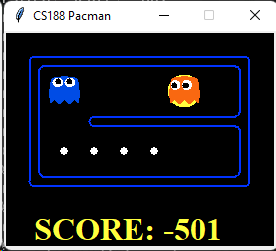
\includegraphics[width=0.5\linewidth]{screenshot002}
\caption{Pacman rushes to the orange ghost and lose the game}
\label{fig:screenshot002}
\end{figure}

I think it's because the minimax algorithm make pacman impossible to go left. If pacman go left, the worst case is that the blue ghost go right, and this will make pacman lose the game. Therefore, the only possible action is to go right, which also make the pacman lose the game.

But for expectimax algorithm, the pacman doesn't consider the worst case, instead, it considers the average case. So if the blue ghost chooses to go down at first move. The pacman will have the chance to eat that four dots. Like the figure below.

\begin{figure}[H]
\centering
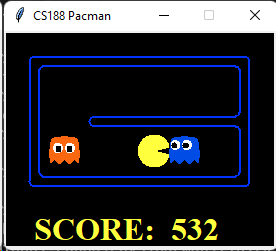
\includegraphics[width=0.5\linewidth]{screenshot004}
\caption{Expectimax algorithm successfully wins trappedClassic}
\label{fig:screenshot004}
\end{figure}

\section{Conclusion}

In this homework, I learn how to write minimax, expectimax, q-learning and approximate q-learning algorithm.

Pacman game is a great example for testing search algorithm and q-learning algorithm.

\end{document}